\documentclass[conference]{IEEEtran}                   \IEEEoverridecommandlockouts                         
% The precending line is only needed ti identify funding in the first footnote.If that is unneeded, please comment it out.
\usepackage{cite}
\usepackage{amsmath,amssymb,amsfonts}                
\usepackage{graphicx}                               
\usepackage{textcomp}                                
\usepackage{xcolor}                                   
\def\BibTeX{{\rm B\kern-.05em{\sc i\kern-.025em b}\kern    -.08em                                                T\kern-.1667em\lower.7ex\hbox{E}\kern-.125emX}}     
\title{                                               
\vspace{1cm}                                             {
\includegraphics[width=0.15\textwidth]{1.jpg} \    \ Platformio Assignment} }                      
\author{sunkari kalpana \\ Roll No:FWC22307\\kalpanamudhiraj@gmail.com}                         
\begin{document}                                        \maketitle                                                \section {ABSTRACT}
This study explores Universal Logic Gates, focusing on NOR and NAND gates as they can implement any Boolean function. The significance of these gates in simplifying digital circuits is emphasized. Additionally, transformer characteristics in AC circuits are briefly analyzed. Key concepts in logic and electrical systems are interlinked.

\section{COMPONENTS}
The required components list s given in Table:I.,
\vspace{0.3cm}
\begin{table} [htbp]
\centering
\begin{tabular}{| c| c | c |} \hline
compoents & value & quality \\\hline
Led & & 1 \\ \hline
Arduino & UNO & 1\\ \hline
jumperwires & & 50 \\ \hline
Breadboard & & 1 \\
\hline
\end{tabular}
\vspace{0.3cm}
\caption{\label{tab:widgets}}
\end{table}
\section{PROCEDURE}
\begin{enumerate}
	\item Convert the Led's to the Arduino uno.
	\item Give the inpts manually using jumper wires.
	\item Truth table for NOT and OR gates.
		\begin{table}[htbp]
			\centering
		


\begin{tabular}{|c|c|c|c|}
\hline
	A & B & A NOR B & A OR B \\
\hline
0 & 0 & 0 & \ldots \\
0 & 0 & 1 & \ldots \\
0 & 1 & 0 & \ldots \\
0 & 1 & 1 & \ldots \\
1 & 0 & 0 & \ldots \\
1 & 0 & 1 & \ldots \\
1 & 1 & 0 & \ldots \\
1 & 1 & 1 & \ldots \\
\hline
\end{tabular}
		
	\vspace{0.1cm}
	\caption{\label{tab:widgets}}
		\end{table}
	\item check the outputs by changing inputs as per truth table.
	\item Execute the arduino code using the pio run command in nvim editor.
	\item After upload the code into hardware setup using arduino IDE platformio.
\end{enumerate}
\section{RESULT}
\begin{enumerate}
	\item Download the code given in the linkbelow and execute them to seethe output as shown in Fig.1.
	\item https://github.com/kalpanasunkari/FWC/tree/main/Assembly
\end{enumerate}

\begin{figure}[h]
	\centering
	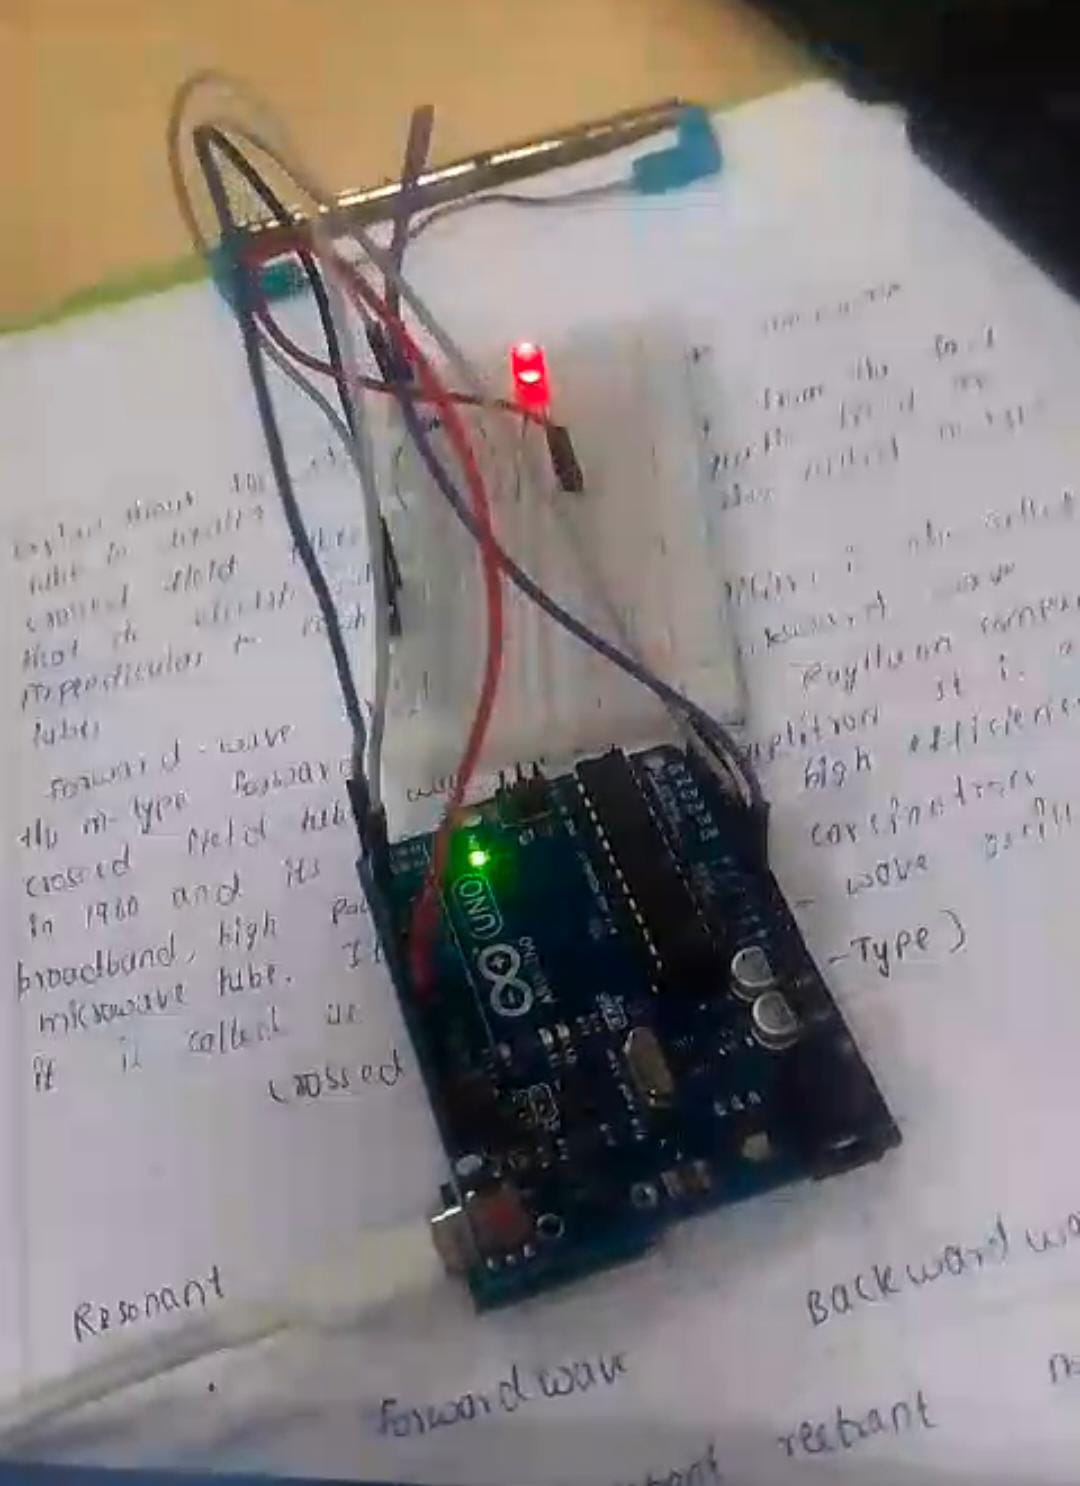
\includegraphics[width=0.4\textwidth]{2.jpg}
	\caption{\label{fig-5:Gates}}
\end{figure}
\section{CONCLUSION}
Hence implementation of platformio using LED id done and verified thriuh truth table.
\end{document}
